\chapter{State模式}
\section{状态模式的概念}
\subsection{定义}
状态(State)模式的定义:对有状态的对象,把复杂的“判断逻辑”提取到不同的状态对象中,允许状态对象在其内部状态发生改变时改变其行为。
\\ 注:
\begin{itemize}
	\item 应用程序中的有些对象可能会根据不同的情况做出不同的行为,我们把这种对象称为有状态的对象,而把影响对象行为的一个或多个动态变化的属性称为状态。
	\item 有状态的的编程解决方案是:将这些所有可能发生的情况全都考虑到,然后使用 if-else 语句来做状态判断,再进行不同情况的处理。但当对象的状态很多时,程序会变得很复杂。而且增加新的状态要添加新的 if-else 语句,这违背了“开闭原则”,不利于程序的扩展。
	\item 状态模式的解决思想是:当控制一个对象状态转换的条件表达式过于复杂时,把相关“判断逻辑”提取出来,放到一系列的状态类当中,这样可以把原来复杂的逻辑判断简单化。
\end{itemize}
\subsection{优点}
\begin{enumerate}
	\item 状态模式将与特定状态相关的行为局部化到一个状态中,并且将不同状态的行为分割开来,满足“单一职责原则”。
	\item 减少对象间的相互依赖。将不同的状态引入独立的对象中会使得状态转换变得更加明确,且减少对象间的相互依赖。
	\item 有利于程序的扩展。通过定义新的子类很容易地增加新的状态和转换。
\end{enumerate}
\subsection{缺点}
\begin{enumerate}
	\item 状态模式的使用必然会增加系统的类与对象的个数。
	\item 状态模式的结构与实现都较为复杂,如果使用不当会导致程序结构和代码的混乱。
\end{enumerate}
\subsection{状态模式的角色}
\begin{enumerate}
	\item State状态:定义一个接口,用以封装环境对象中的特定状态所对应的行为,是那些处理内容依赖状态的方法的结合。
	\item ConcreteState具体状态:实现抽象状态所对应的行为。
	\item Context状况/上下文:也称为上下文,它定义了客户感兴趣的接口,维护一个当前状态,并将与状态相关的操作委托给当前状态对象来处理。
\end{enumerate}
\subsection{应用场景}
\begin{enumerate}
	\item 当一个对象的行为取决于它的状态,并且它必须在运行时根据状态改变它的行为时,就可以考虑使用状态模式。
	\item 一个操作中含有庞大的分支结构,并且这些分支决定于对象的状态时。
\end{enumerate}
\section{状态模式实现——例一}
\begin{table}[!h]
	\begin{tabular}{|l|l|}
		\hline
		名字&说明\\
		\hline
		State&金库状态的接口\\
		\hline
		DayState&白天状态的类,实现了State接口\\
		\hline
		NightState&晚上状态的类,实现了State接口\\
		\hline
		Context&管理金库状态,并与警报中心联系的接口\\
		\hline
		SafeFrame&实现了Context接口,内部持有按钮和画面显示等UI信息\\
		\hline
		Main&测试行为类\\
		\hline
	\end{tabular}
\end{table}
\begin{figure}[!h]
	\centering
	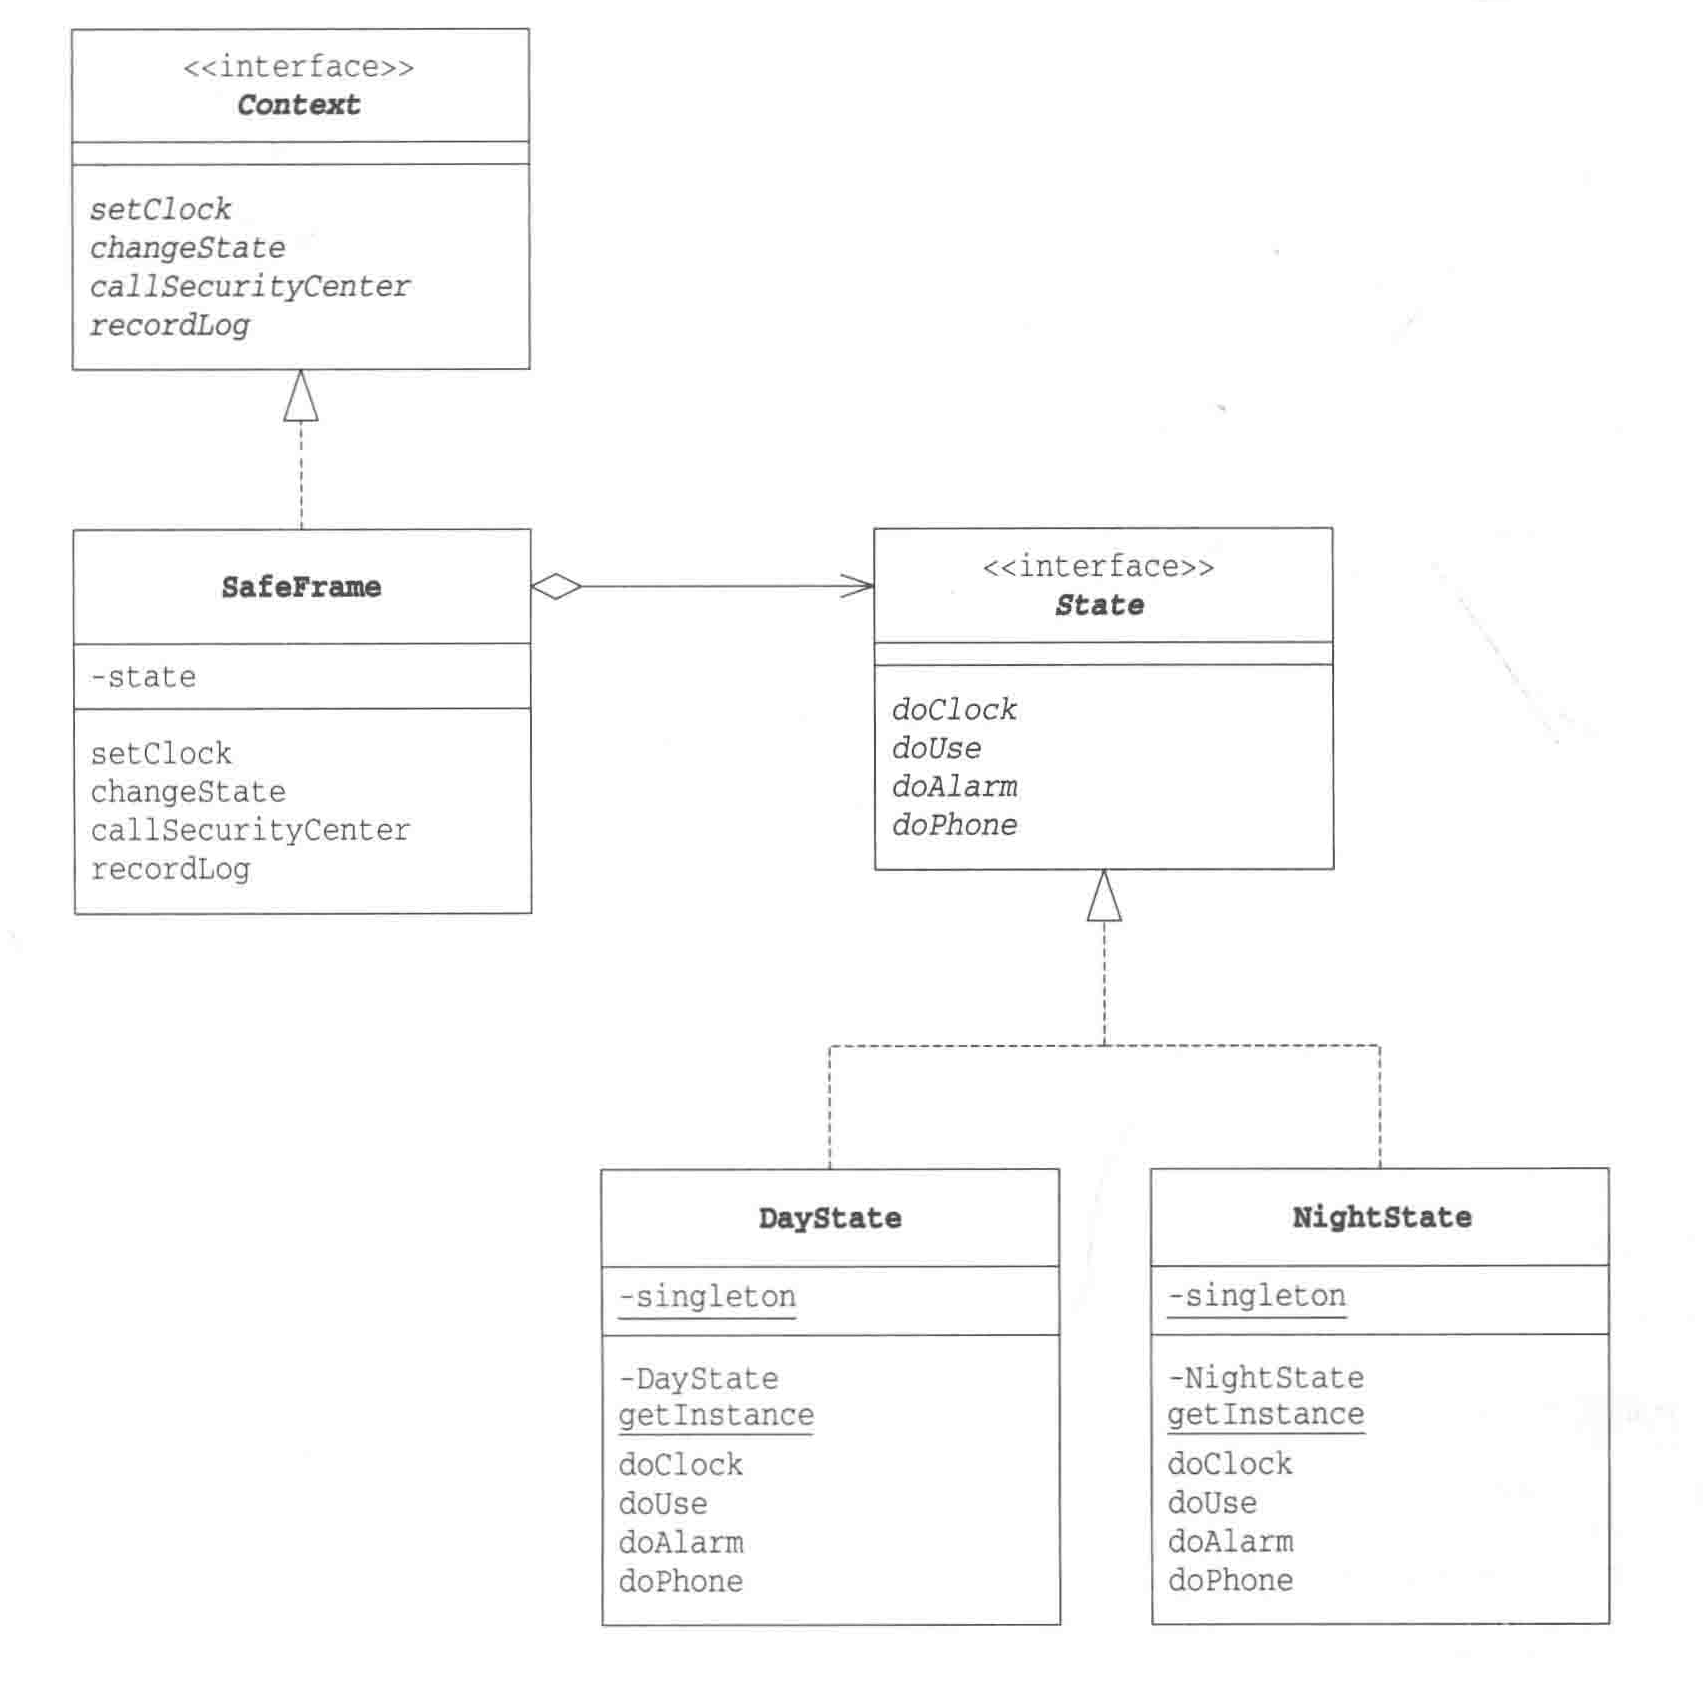
\includegraphics[width=0.8\textwidth]{image/19-1}
	\caption{状态模式类图}
\end{figure}
\begin{lstlisting}
public interface State {
	void doClock(Context context, int hour);
	void doUse(Context context);
	void doAlarm(Context context);
	void doPhone(Context context);
}
public interface Context {
	void setClock(int hour);
	void changeState(State state);
	void callSecurityCenter(String msg);
	void recordLog(String msg);
}
\end{lstlisting}
\begin{lstlisting}
public class DayState implements State {
	private static DayState singleton = new DayState();
	private DayState() {}
	public static State getInstance() {
		return singleton;
	}
	public void doClock(Context context, int hour) {
		if (hour < 9 || 17 <= hour) {
			context.changeState(NightState.getInstance());
		}
	}
	public void doUse(Context context) {
		context.recordLog("使用金库(白天)");
	}
	public void doAlarm(Context context) {
		context.callSecurityCenter("按下警铃(白天)");
	}
	public void doPhone(Context context) {
		context.callSecurityCenter("正常通话(白天)");
	}
	public String toString() {
		return "[ 白天 ]";
	}
}
\end{lstlisting}
\begin{lstlisting}
public class NightState implements State {
	private static NightState singleton = new NightState();
	private NightState() {}
	public static State getInstance() {
		return singleton;
	}
	public void doClock(Context context, int hour) {
		if (9 <= hour && hour < 17) {
			context.changeState(DayState.getInstance());
		}
	}
	public void doUse(Context context) {
		context.callSecurityCenter("紧急:晚上使用金库!");
	}
	public void doAlarm(Context context) {
		context.callSecurityCenter("按下警铃(晚上)");
	}
	public void doPhone(Context context) {
		context.recordLog("晚上的通话录音");
	}
	public String toString() {
		return "[ 晚上 ]";
	}
}
\end{lstlisting}
\begin{lstlisting}
// 实现了 Context 接口,使用 GUI 实现警报系统界面
public class SafeFrame extends Frame implements ActionListener, Context {
	private TextField textClock = new TextField(60);
	private TextArea textScreen = new TextArea(10, 60);
	private Button buttonUse = new Button("Use");
	private Button buttonAlarm = new Button("Alarm");
	private Button buttonPhone = new Button("Call");
	private Button buttonExit = new Button("Exit");
	private State state = DayState.getInstance();
	
	public SafeFrame(String title) throws HeadlessException {
		super(title);
		setBackground(Color.lightGray);
		setLayout(new BorderLayout());
		add(textClock, BorderLayout.NORTH);
		textClock.setEditable(false);
		add(textScreen, BorderLayout.CENTER);
		textScreen.setEditable(false);
		Panel panel = new Panel();
		panel.add(buttonUse);
		panel.add(buttonAlarm);
		panel.add(buttonPhone);
		panel.add(buttonExit);
		add(panel, BorderLayout.SOUTH);
		pack();
		show();
		buttonUse.addActionListener(this);
		buttonAlarm.addActionListener(this);
		buttonPhone.addActionListener(this);
		buttonExit.addActionListener(this);
	}
	
	//设置时间
	public void setClock(int hour) {
		String clockString = "现在时间是:";
		if (hour < 10) {
			clockString += "0" + hour + ":00";
		} else {
			clockString += hour + ":00";
		}
		System.out.println(clockString);
		textClock.setText(clockString);
		state.doClock(this, hour);
	}
	//改变状态
	public void changeState(State state) {
		System.out.println("从" + this.state + "状态变为了" + state + "状态。");
		this.state = state;
	}
	
	//联系警报中心
	public void callSecurityCenter(String msg) {
		textScreen.append("call! " + msg + "\n");
	}
	
	//在警报中心留下记录
	public void recordLog(String msg) {
		textScreen.append("recode ... " + msg + "\n");
	}
	
	public void actionPerformed(ActionEvent e) {
		System.out.println(e.toString());
		if (e.getSource() == buttonUse) {
			state.doUse(this);
		} else if (e.getSource() == buttonAlarm) {
			state.doAlarm(this);
		} else if (e.getSource() == buttonPhone) {
			state.doPhone(this);
		} else if (e.getSource() == buttonExit) {
			System.exit(0);
		} else {
			System.out.println("?");
		}
	}
}
\end{lstlisting}
\begin{lstlisting}
public class Main {
	public static void main(String[] args) {
		SafeFrame frame = new SafeFrame("state Sample");
		while (true) {
			for (int hour = 0; hour < 24; hour++) {
				frame.setClock(hour);
				try {
					Thread.sleep(1000);
				} catch (InterruptedException e) {
				}
			}
		}
	}
}
\end{lstlisting}
\section{状态模式实现——例二}
\begin{figure}[!h]
	\centering
	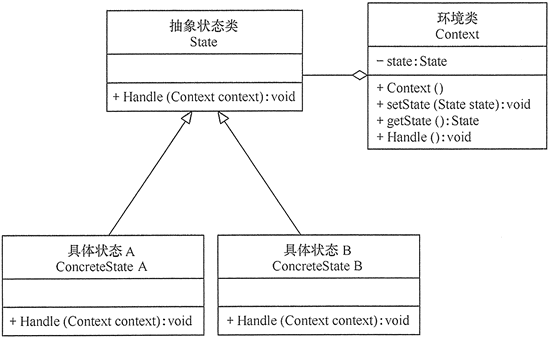
\includegraphics[width=0.8\textwidth]{image/19-2}
	\caption{状态模式的结构图}
\end{figure}
\begin{lstlisting}
//抽象状态类
abstract class State {
	public abstract void Handle(Context context);
}

//具体状态A类
class ConcreteStateA extends State {
	public void Handle(Context context) {
		System.out.println("当前状态是 A.");
		context.setState(new ConcreteStateB());
	}
}

//具体状态B类
class ConcreteStateB extends State {
	public void Handle(Context context) {
		System.out.println("当前状态是 B.");
		context.setState(new ConcreteStateA());
	}
}
\end{lstlisting}
\begin{lstlisting}
//环境类
class Context {
	private State state;
	//定义环境类的初始状态
	public Context() {
		this.state = new ConcreteStateA();
	}
	//设置新状态
	public void setState(State state) {
		this.state = state;
	}
	//读取状态
	public State getState() {
		return (state);
	}
	//对请求做处理
	public void Handle() {
		state.Handle(this);
	}
}
\end{lstlisting}
\begin{lstlisting}
public class StatePatternClient {
	public static void main(String[] args) {
		Context context = new Context();    //创建环境
		context.Handle();    //处理请求
		context.Handle();
		context.Handle();
		context.Handle();
	}
}
\end{lstlisting}
\begin{lstlisting}
//output
当前状态是 A.
当前状态是 B.
当前状态是 A.
当前状态是 B.
\end{lstlisting}
\section{模式扩展}
在有些情况下,可能有多个环境对象需要共享一组状态,这时需要引入享元模式,将这些具体状态对象放在集合中供程序共享。
\par 共享状态模式的不同之处是在环境类中增加了一个 HashMap 来保存相关状态,当需要某种状态时可以从中获取。
\begin{figure}[!h]
	\centering
	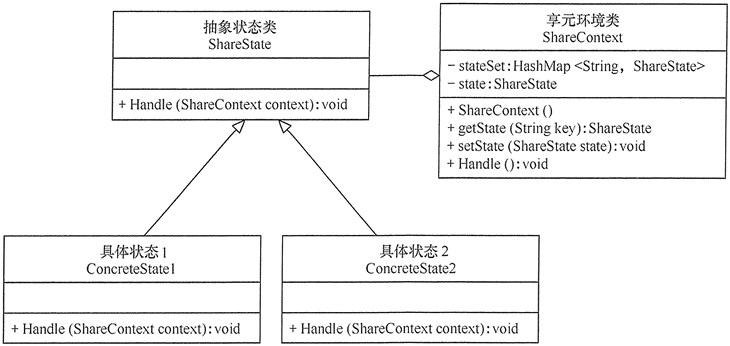
\includegraphics[width=0.8\textwidth]{image/19-3}
	\caption{共享状态模式的结构图}
\end{figure}
\begin{lstlisting}
//环境类
class ShareContext {
	private ShareState state;
	private HashMap<String, ShareState> stateSet = new HashMap<String, ShareState>();
	public ShareContext() {
		state = new ConcreteState1();
		stateSet.put("1", state);
		state = new ConcreteState2();
		stateSet.put("2", state);
		state = getState("1");
	}
	//设置新状态
	public void setState(ShareState state) {
		this.state = state;
	}
	
	//读取状态
	public ShareState getState(String key) {
		ShareState s = (ShareState) stateSet.get(key);
		return s;
	}
	//对请求做处理
	public void Handle() {
		state.Handle(this);
	}
}
\end{lstlisting}
\begin{lstlisting}
//抽象状态类
abstract class ShareState {
	public abstract void Handle(ShareContext context);
}

//具体状态1类
class ConcreteState1 extends ShareState {
	public void Handle(ShareContext context) {
		System.out.println("当前状态是: 状态1");
		context.setState(context.getState("2"));
	}
}

//具体状态2类
class ConcreteState2 extends ShareState {
	public void Handle(ShareContext context) {
		System.out.println("当前状态是: 状态2");
		context.setState(context.getState("1"));
	}
}
\end{lstlisting}
\begin{lstlisting}
public class FlyweightStatePattern {
	public static void main(String[] args) {
		ShareContext context = new ShareContext(); //创建环境
		context.Handle(); //处理请求
		context.Handle();
		context.Handle();
		context.Handle();
	}
}
\end{lstlisting}
\section{扩展思路}
\begin{enumerate}
	\item 分而治之:在State中,用类表示状态,分解了问题;
	\item 依赖状态的处理:在State中设置的所有方法都是依赖状态的处理;
	\item 管理状态迁移:可以在Context委托给State处理,将状态迁移看为依赖状态的处理,但有优缺点:
	\begin{itemize}
		\item 优点:逻辑清晰;
		\item 缺点:各个类之间依赖性强;
	\end{itemize}
	解决办法:将所有的状态迁移交给Context(结合Mediator)。
	\item 不会自相矛盾:设置状态要小心,变量之间不能矛盾;
	\item 易于增加新的状态,但增加其他“依赖于状态的处理”困难,并且要注意
	状态转移的处理;
\end{enumerate}
\section{相关设计模式}
\begin{enumerate}
	\item Singleton模式:Singleton模式会出现在ConcreteState中;
	\item Flyweight模式:可以像例二一样共享ConcreteState角色。
\end{enumerate}